\section{Quick Overview}

\subsection{Includes}

\begin{lstlisting}
#include <iosfwd> 	// Only the declaration for input and output streams
#include <istream>  // Implementation of input stream
#include <ostream>  // Implementation of output stream
#include <iostream> // std::cout, std::cin, std::cerr
#include <cctype>   // Functions: std::tolower(c), std::isupper(c)
#include <string>   // Strings
#include <array>
#include <cctype> // lowercase, isalpha,isblank, toupper
#include <vector>
#include <numeric>  // std::iota
#include <iterator> // std::count, std::accumulate, std::distance, std::for_each
#include <functional> // greater, less, logical_and
#include <deque>    // std::deque<T>
#include <list>
#include <forward_list> // std::forward_list<T>
#include <stack>
#include <queue>
#include <stack> // std::priority_queue
#include <set>
#include <map>
#include <unordered_set> // std::unordered_set --> Hashed
#include <unordered_map> // std::unordered_map --> Hashed
#include <memory> // std::unique_ptr / std::shared_ptr (smart pointer)
#include <stdexcept> // out_of_range, runtime_error, range_error
\end{lstlisting}

\pagebreak

\subsection{ASCII Table}
\begin{figure}[h!]
  \center
  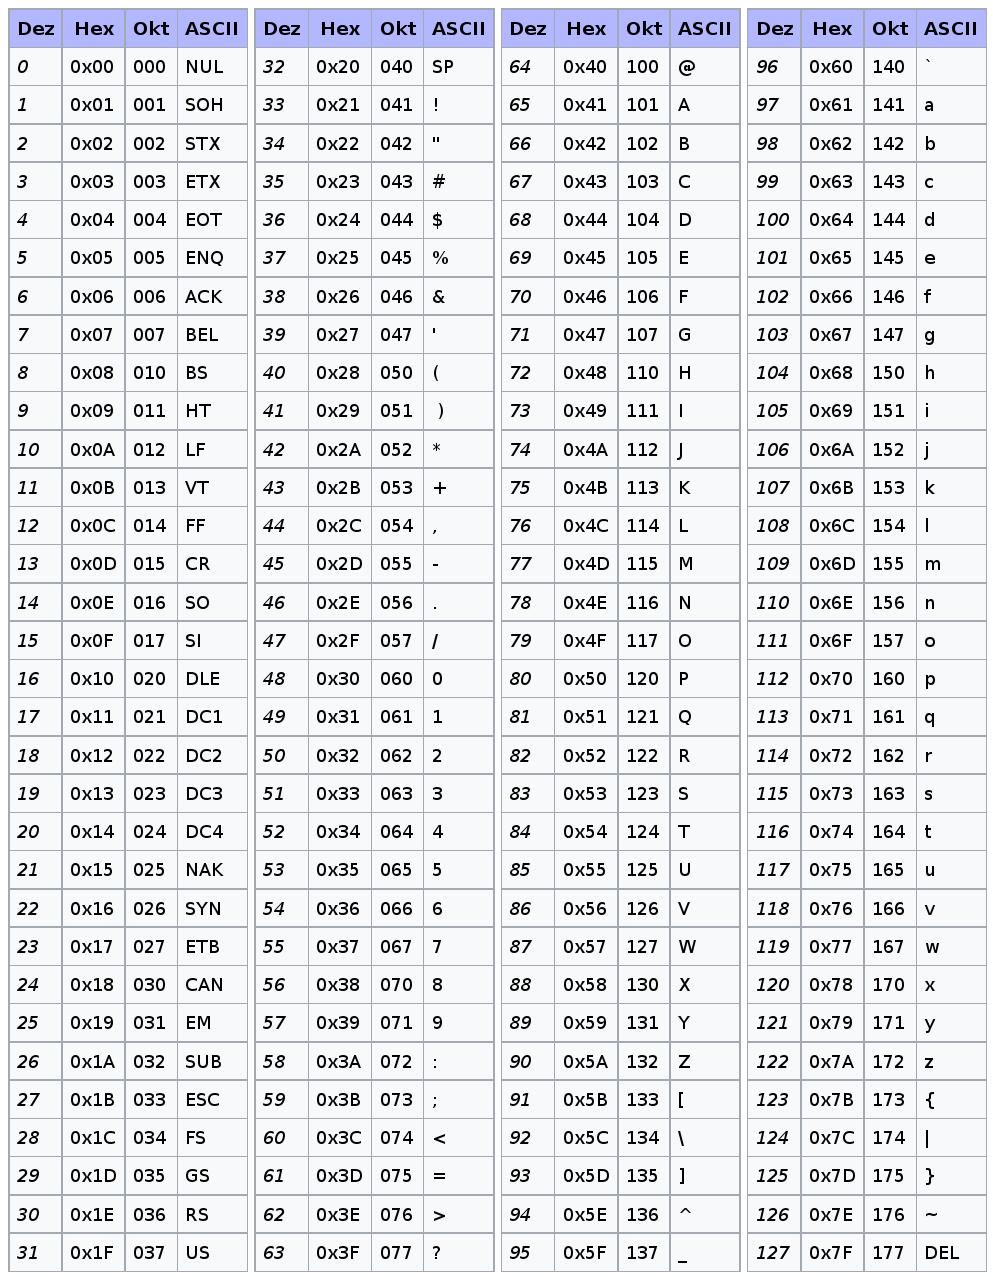
\includegraphics[width=0.9\linewidth]{ascii_table}
  \caption{ASCII Table}
\end{figure}

\pagebreak
